\section{Durchführung}
\label{sec:Durchführung}
Der prinzipielle Aufbau einer Wärmepumpe wurde bereits in Abschnitt \ref{sec:Versuchsaufbau} erläutert. Die im Versuch verwendete Wärmepumpe ist in Abbildung \ref{fig:bild2} schematisch dargestellt.
\begin{figure}
  \centering
  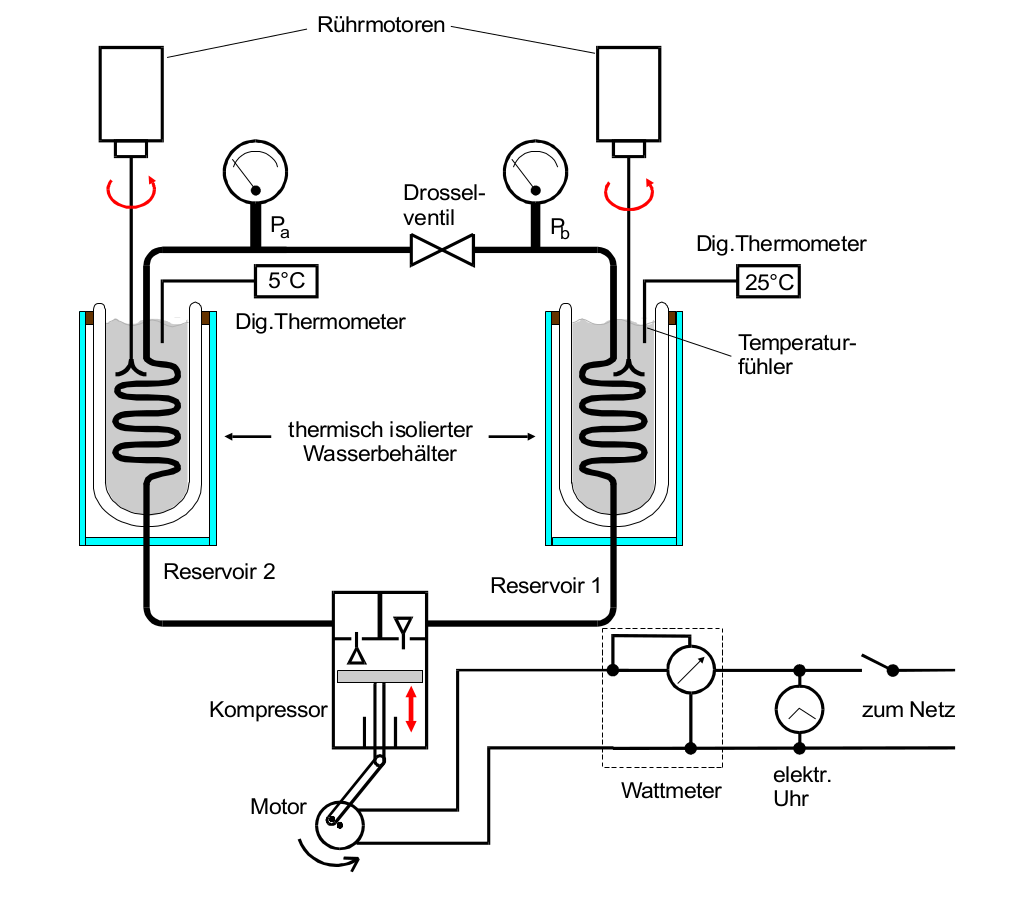
\includegraphics[width=\textwidth]{content/messapparatur.png}
  \caption{Schematischer Aufbau der Messapparatur \cite{Anleitung}}
  \label{fig:bild2}
\end{figure}

Die Rührmotoren dienen hier lediglich dazu, dass das Wasser in den beiden Reservoiren permament durchgemischt wird, sodass eine homogene Temperatur in den Reservoiren erreicht wird.
Zusätzlich sind jeweils ein Manometer und ein elektronisches Thermometer zur Messung von Druck und Temperatur auf beiden Seiten der Wärmepumpe angebracht.
Außerdem kann die Leistungsaufnahme des Kompressors mittels eines Wattmeters abgelesen werden.

Zu Beginn des Versuchs werden beide Reservoire mit gleichwarmen Wasser gefüllt (jeweils 4 Liter bei etwa 20°C).
Beim Einbau der beiden Reservoire in die Versuchsapparatur ist darauf zu achten, dass die Reservoire dicht an die Apparatur anschließen, sodass ein Wärmeaustausch mit der Umgebung weitmöglichst verringert wird.

Sämtliche Kupferleitungen sowie die beiden Reservoire sind isoliert, sodass auch hier der Wärmeaustausch mit der Umgebung verringert wird.
Zu Beginn des Versuchs werden nun beidseitig Temperatur und Druck gemessen. Nun wird der Kompressor eingeschaltet und minütlich werden die Leistungsaufnahme des Kompressors, sowie beide Drücke und Temperaturen notiert, bis entweder im kälteren Reservoir 0°C, oder im wärmeren Reservoir 50°C erreicht werden.
Die spezifische Wärmekapazität von Kupferrohren und den beiden Reservoiren wird zusätzlich noch benötigt.
